\chapter {Protocole Expérimental}


\section{Matériel utilisé}

\subsection{Déplacement du robot}

Le robot est équipé de trois roues, desquelles les symétriques
arrières sont motorisés et responsables pour le déplacement
motrice. Au même temps que la dernière sert à donner un support pour
la partie derrière du châssis. Les moteurs sont contrôlés à
partir de commandes sériel, préétablis pour le fabricant, qui
définissent la vitesse de roulement. La combinaison des rotations
des deux roues motorises dans les deux sens possibles permets au
robot d'avoir les comportements suivants:

\begin {itemize}
\item Déplacement en ligne droite : deux roues roulant avec la même vitesse et dans le même sens.

\item Déplacement en arc de cercle : différence entre les vitesses des roues.

\item Rotation : deux roues à la même vitesse, mais avec de sens différents.
\end{itemize}

Finalement, la combinaison de ces mouvements permet au robot de
accéder n'importe quelle position de l’espace.


Le design de l'architecture a permis de définir les unités de traitement et la communication entre elles. La définition des unités de traitement suit le découpage du pipeline de reconnaissance avec des nœuds dédiés pour la segmentation, l'extraction de features, la classification, mais également le contrôle du robot.

L'interfaçage matériel-logiciel a été réalisé sur l'environnement ROS - Robot Operating System. En plus d'outils d'affichage, ROS rassemble des librairies d'acquisition d'images RGB-D, OpenNi 2 et Freenect, ainsi qu'une librairie de traitement de nuage de points, PCL.
De plus, sa structure en nœuds a permis une implémentation modulaire et directe du système décrit \celine{au chapitre \ref{}}, ainsi que de gérer la communication entre l'ordinateur portable et le processeur embarqué sur le robot.

L'image \celine{ \ref{}} présente l'architecture ainsi que le flux d'information à travers des nœuds.\celine{ Mets plutôt l'image en annexe, ca gagnera de la place}

\section{Setup expérimental}
Pour évaluer les capacités de reconnaissance du robot, vingt objets de tailles et formes diverses ont été choisis. Ils s'agit d'objets typiques qui peuvent être faciliment retrouvés dans un laboratoire ou un bureau. Une liste complète des objets figure en annexe \celine{\ref{}}. Ensuite, nous avons effectué un tour complet de l'objet avec le robot en sauvegardant les nuage de point et en extrayant les features VFH pour huit positions différentes écartées de 45 degrés. La position correspondent à l'angle zéro a été choisie de manière aléatoire en alignant un des axes de l'objet avec celui du capteur. \celine{Regarde ma remarque à la figure \ref{fig:setup_expe}}

\begin{figure}[H]
	\subfloat{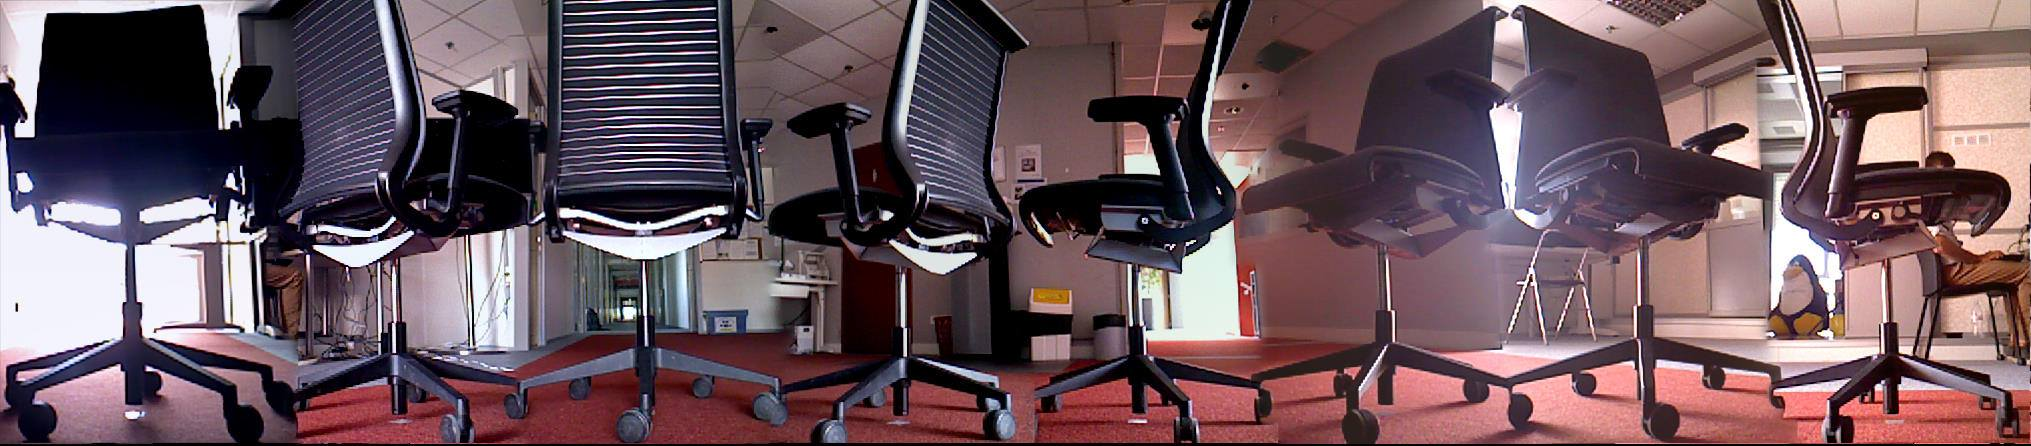
\includegraphics[width=\textwidth]{chair_db.jpg}}		
	\caption{\celine{Pense à toujours mettre une légende à tes figures, et à donner sa référence dans le texte}}
	\label{fig:setup_expe}
\end{figure}

\section{Résultats expérimentaux}
\subsection{Comparaison à la reconnaissance mono-vue}
Une première évaluation consiste à faire un tour complet autour de l'objet à reconnaitre pour quatre positions angulaires différentes : $0, 45, 90$ et une dernière choisie de manière aléatoire pour chaque objet. Le robot fait le tour à une vitesse de $0.35 \pm 0.1 m/s$ à une distance de $1.5m$, en enregistrant des images à $1hz$, ansi, une expérience typique est constituée d'environ $25$  images d'angle différent et prendre $25 \pm 3$ seconds. 

Un expérience typique est illustrée dans l'image \ref{fig:resultats_expe} :

\begin{figure}[H]
	\subfloat{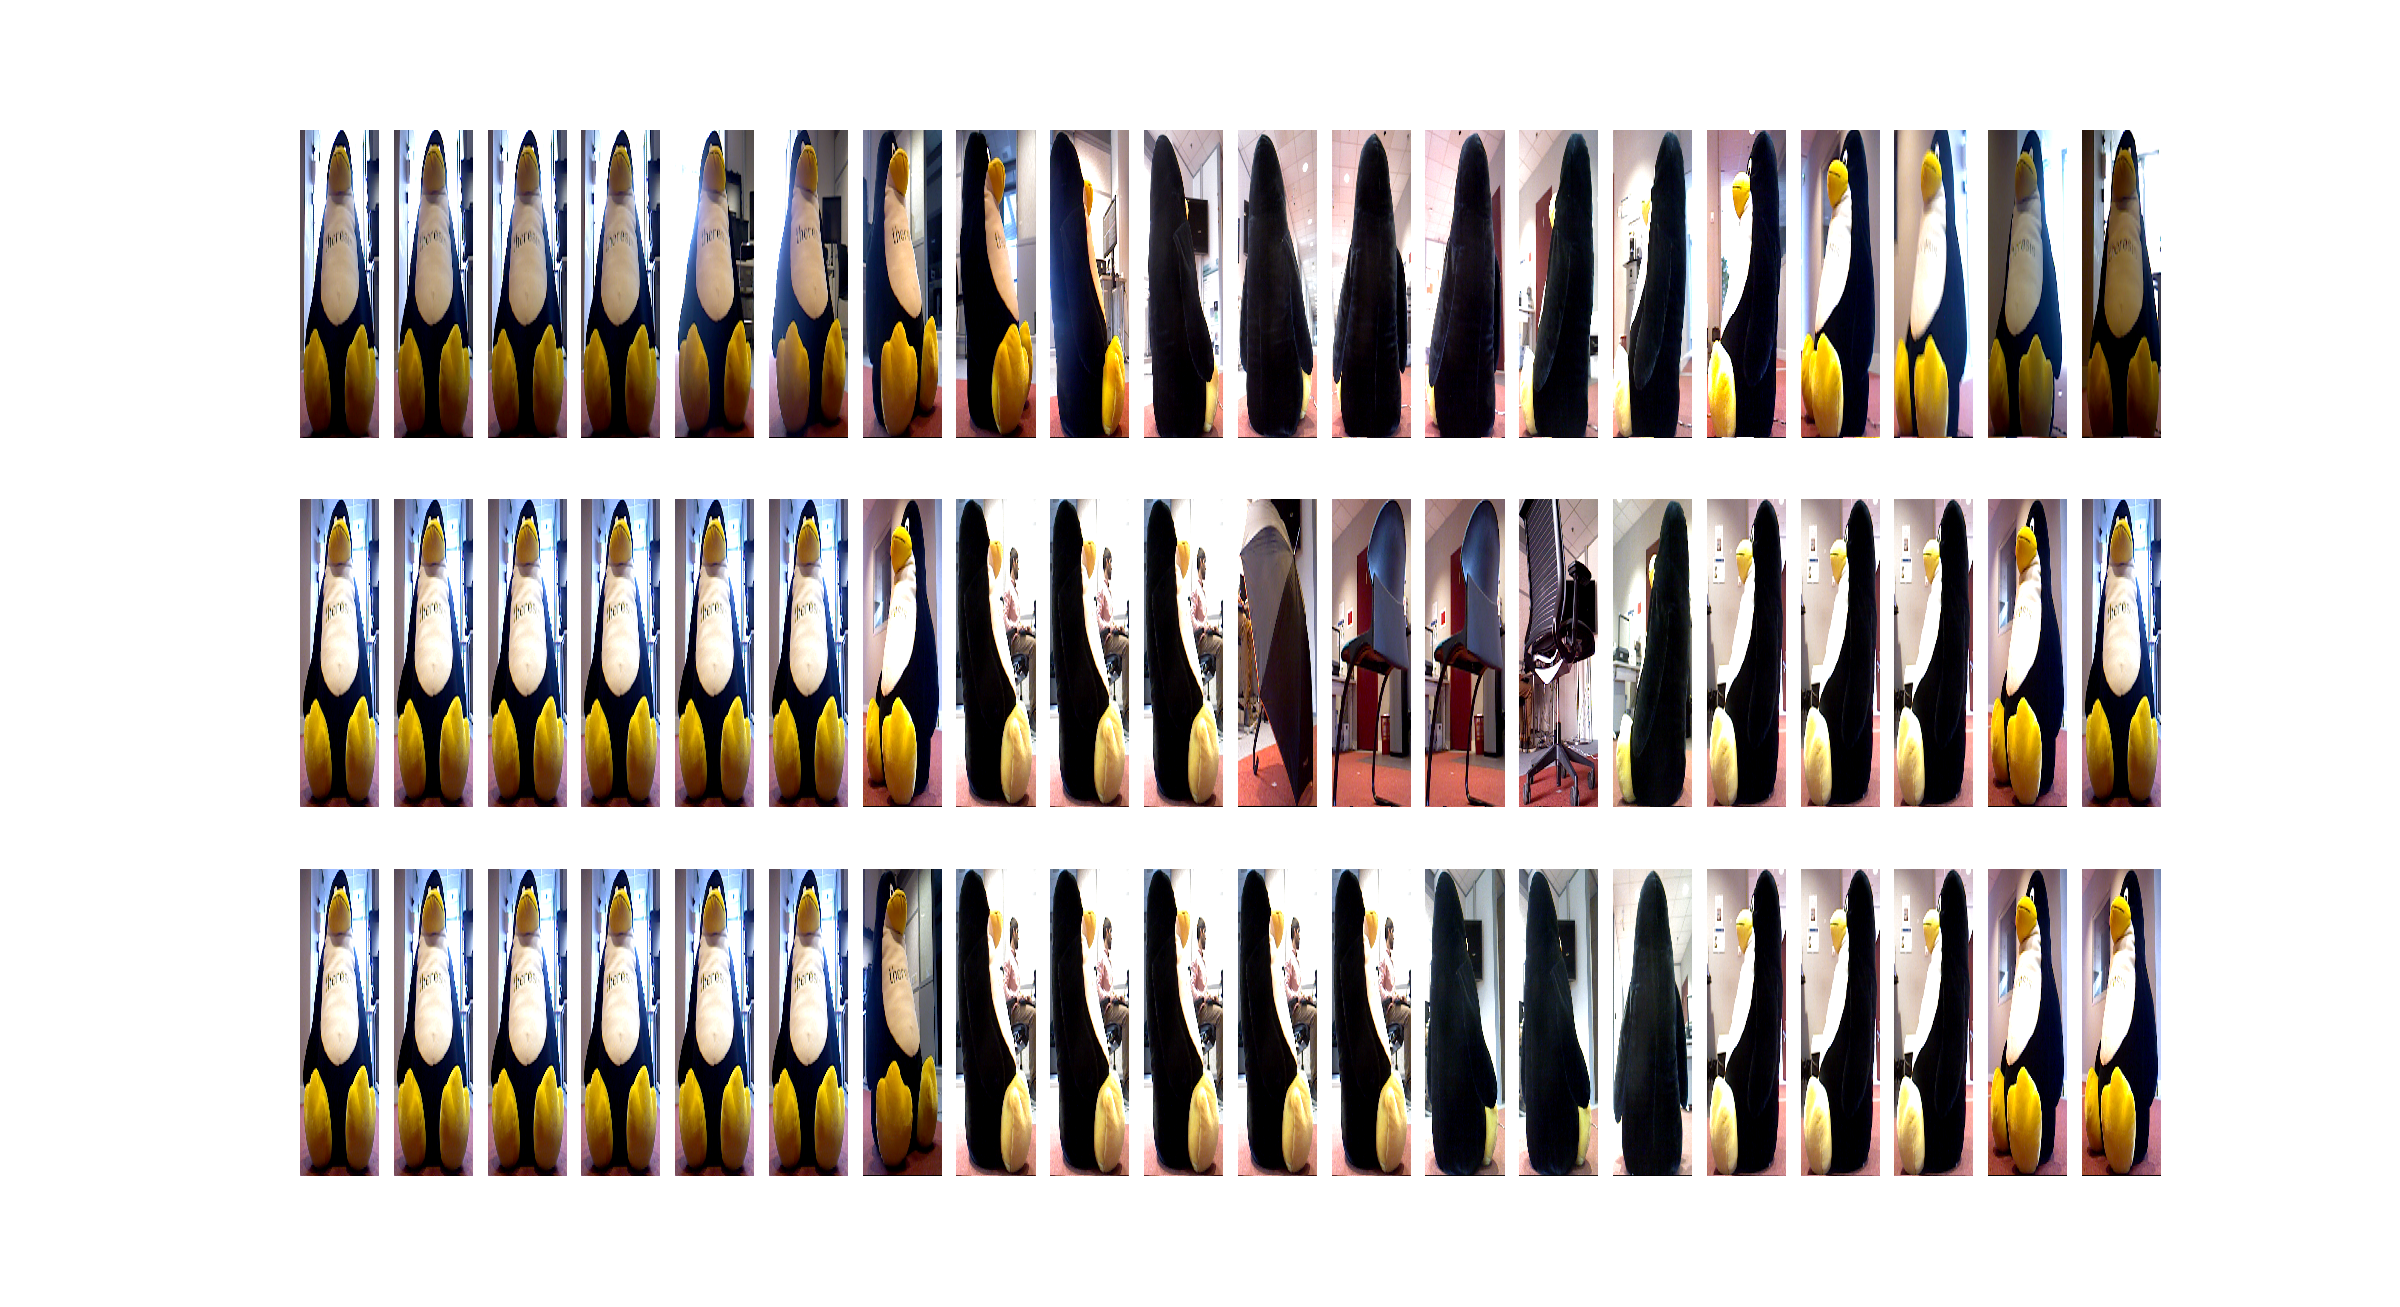
\includegraphics[width=\textwidth]{hmm_example.png}}	
			\caption{\celine{Tu devrais ajouter sur le côté de l'image que c'est l'image observée, l'image la plus proche par la reco mono-vue, et l'image la plus proche avec les HMM (même si tu le répète dans le texte, ca permet de comprendre la figure directement)}}
	\label{fig:resultats_expe}
\end{figure}

La première ligne correspond à la séquence d'images vues par le robot à chaque instant de temps, et donc, l'objet à être reconnu. La seconde ligne, donnée par l'algorithme de reconnaissance, équivaut à la vue la plus probable de l'objet reconnue par le K-plus proches voisins. Il est intéressant remarquer que l'invariance à rotation du descripteur trompe l'estimation de l'orientation en prenant son correspond énantiomorphe dans le premier carré rouge. Autrement, le dos du pinguin étant une grande surface presque plane, il est partiellement retiré par l'étape de segmentation. Ainsi, le nuage de points résultant de ce point de vue n'est pas suffisamment complet pour caractériser correctement l'objet, ce qui induit une mauvaise reconnaissance dans le carré bleu. Au final, on remarque que le traitement apporté par la chaîne de Markov cachée permet de corriger les problèmes d'une base de donnée relativement sparse avec des possibles erreus de segmentation, permettant la correction simultanée de la reconnaissance de l'objet et de son orientation. 

cela correspond à avoir une base
On utilise ensuite trois ratios différentes pour exprimer la reconnaissance d'objets, la reconnaissance de vue et la suivi des reconnaissances par la chaîne de Markov cachée.
Finalement,  est affichée

\begin{figure}[H]
	\subfloat{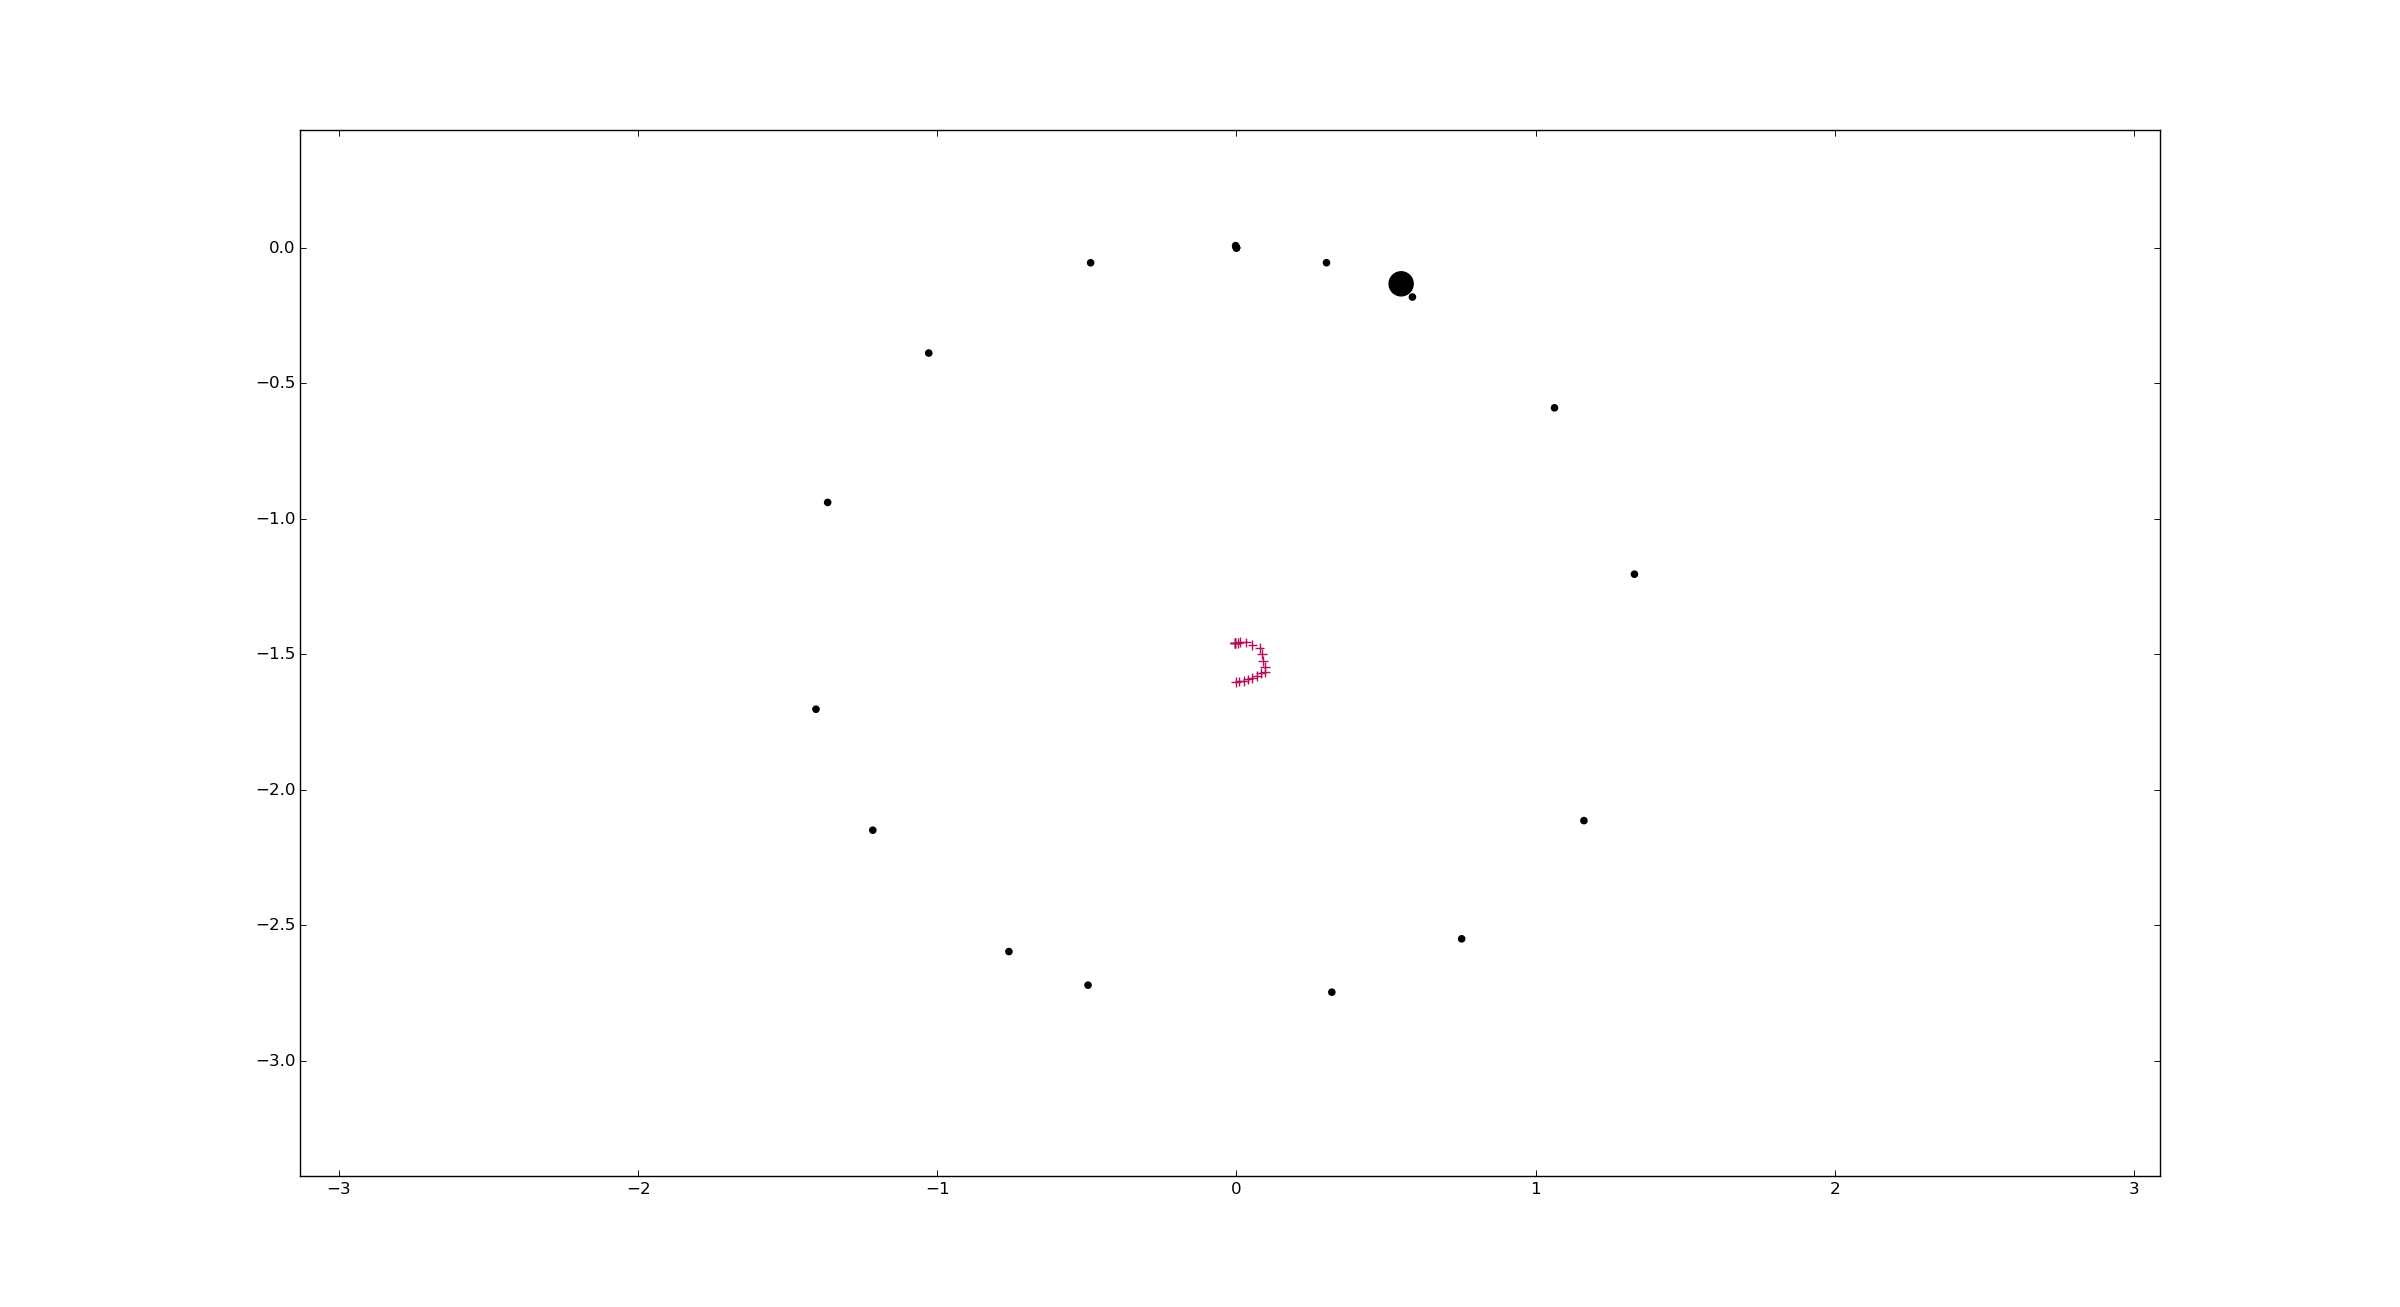
\includegraphics[width=\textwidth]{hmm_mov.png}}		
\end{figure}


{\color{green}
Dans le premier tableaux on retrouve le résultats de la reconnaissance donné par la comparaison des histogrammes provenant du *plus proche voisin*. Ce résultat estime la capacité de distinguer deux objets quelconques, en autre mots, cette capacité viens de la représentativité des descripteurs utilisés et l'efficacité de la mesure de similarité entre histogrammes.
}

\subsection{Robustesse à l'occlusion}

\subsection{Suivi et reconnaissance multi-cibles}

%\begin{figure}[H]
%	\subfloat{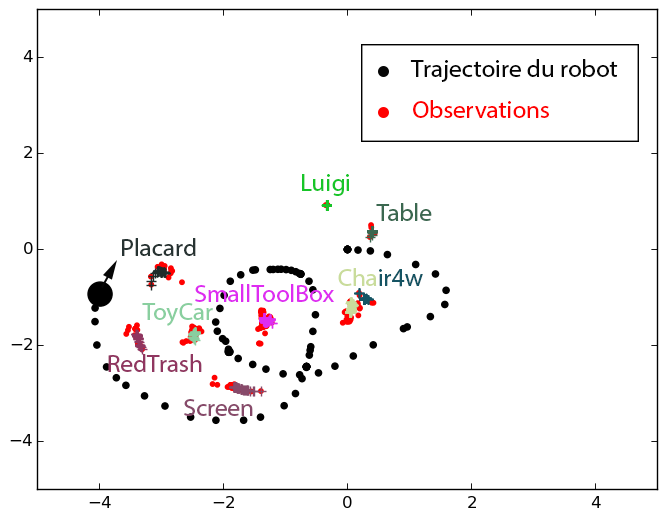
\includegraphics[width=\textwidth]{map.png}}		
%\end{figure}

\section{Problèmes rencontrés}

\subsubsection{Problèmes de déplacement}

La roulette de support originalement installée avait deux axes de
rotation. Pourtant, quelques mouvements de rotation du robot alignent
la roulette orthogonalement au sens du prochain mouvement ce qui crées
une torche parasite que perturbe la trajectoire voulue. Une tentative
frustrée d'installer une bille omnidirectionnelle à roulement, qui se
bloquait sur la moquette avec le poids du robot, a fait que
l'originale était réinstallée. Une deuxième solution serait d'interdire
certains mouvements du robot pour éviter cette déviation.